% !TeX root = ../main.tex
\documentclass[./../main.tex]{subfiles}

\begin{document}

Ứng dụng được phát triển từ nhu cầu thực tế của thành viên trong nhóm, các cá nhân thích đọc truyện tranh. Trong đó, việc đọc truyện với UI/UX tốt, chất lượng tốt là mục tiêu của nhóm trong việc phát triển. Với vai trò và mục tiêu trên, nhóm đã phân tích vấn đề thành các đơn vị nhỏ hơn sau.

\subsection{Đối tượng sử dụng}

Hệ thống có 3 đối tượng sử dụng chính.

\begin{description}
	\item[Khách vãng lai đọc truyện] Bất kỳ người dùng truy cập website, ứng dụng di động có thể đọc các truyện trên hệ thống. Mục đích đối với nhóm người này là có thể nhanh chóng đọc truyện được thông qua việc chia sẻ của bạn bè thông qua mạng xã hội, đường dẫn liên kết hay chỉ với tên của Website.
	\item[Người dùng đọc truyện] Người dùng của hệ thống cho phép đọc truyện, theo dõi, nhận thông báo,...và các tính năng khác của hệ thống. Nhóm người này có mục đích thường xuyên đọc và theo dõi truyện từ  hệ thống muốn nhận được thêm các thông báo khi có nội dung mới được đưa ra. Đi kèm với đó là sử dụng các tính năng khác mang tính cá nhân như là theo dõi được lịch sử đọc truyện, lưu lại truyện hay đọc,…
	\item[Quản trị viên] Người quản trị nội dung hệ thống, người dùng. Đồng thời cũng là người tạo ra các truyện dựa trên sự ủy quyền của tác giả. Nhóm người này có mục đích chính là quản trị hệ thống cả về nội dung và con người để đảm bảo hệ thống diễn ra đảm bảo nhất. Các nội dung được đăng trên hệ thống cần thông qua nhóm người dùng này.
\end{description}

\subsection{Yêu cầu chức năng}

Dựa vào các nhóm người dùng trên, các yêu cầu chức năng được đặt ra là
\begin{itemize}
	\item Cho phép xem, đọc nội dung của của truyện tranh.
	\item Tìm hiểu thông tin về tác giả.
	\item Cho tìm kiếm truyện.
	\item Bình luận về truyện.
	\item Nhận thông báo về truyện.
	\item Lưu lại các bộ truyện yêu thích.
	\item Đăng nhập, đăng ký
	\item Hiển thị các trang truyện theo đúng thứ tự
	\item Người dùng có thể chuyển chap, chỉnh chế độ đọc, ...
	\item Lưu trữ danh sách yêu thích
	\item Đăng truyện mới
	\item Đăng chap truyện mới
	\item Dark mode
	\item Báo cáo lỗi truyện
	\item Đa ngôn ngữ (i18next)
	\item Nhận thông báo chap mới
\end{itemize}

\subsection{Yêu cầu phi chức năng}

Dựa vào nhu cầu của người dùng, nhóm định nghĩa được 4 yêu cầu phi chức năng cho sản phẩm.

\subsubsection{Tính khả dụng}

Đáp ứng > 90\% trên toàn bộ mẫu người sử dụng dùng có thể...
\begin{itemize}
	\item Có thể sử dụng hệ thống trong 5 phút.
	\item Đăng ký trong vòng 5 phút.
	\item Đăng nhập trong vòng 1 phút.
	\item Tìm kiếm truyện và đọc được truyện trong vòng 1 phút.
\end{itemize}

\subsubsection{Tính sẵn sàng}

Đáp ứng thời gian vận hành liên tục trên 98\%.

\subsubsection{Hiệu suất}

\begin{itemize}
	\item Đáp ứng ít nhất cho 5.000 CCU.
	\item Đáp ứng 95\% số yêu cầu dưới 5s.
	\item Trung bình thời gian phản hồi mỗi yêu cầu là dưới 2s.
\end{itemize}

\subsubsection{Bảo mật}

Khả năng bảo vệ hệ thống trước tấn công DDoS, hạn chế các lỗ hổng nguy hiểm. Đảm bảo bảo mật về thông tin cá nhân.

\subsection{Mô hình ca sử dụng}

Dựa vào các yêu cầu đối với các nhóm đối tượng ở trên, nhóm đã mô hình hóa thành các Tác nhân đối với hệ thống.

Ngoài ra, Firebase được triển khai như một hệ thống ngoài của hệ thống nên sẽ được coi là một tác nhân cần tương tác với hệ thống.

\begin{figure}[H]
	\centering
	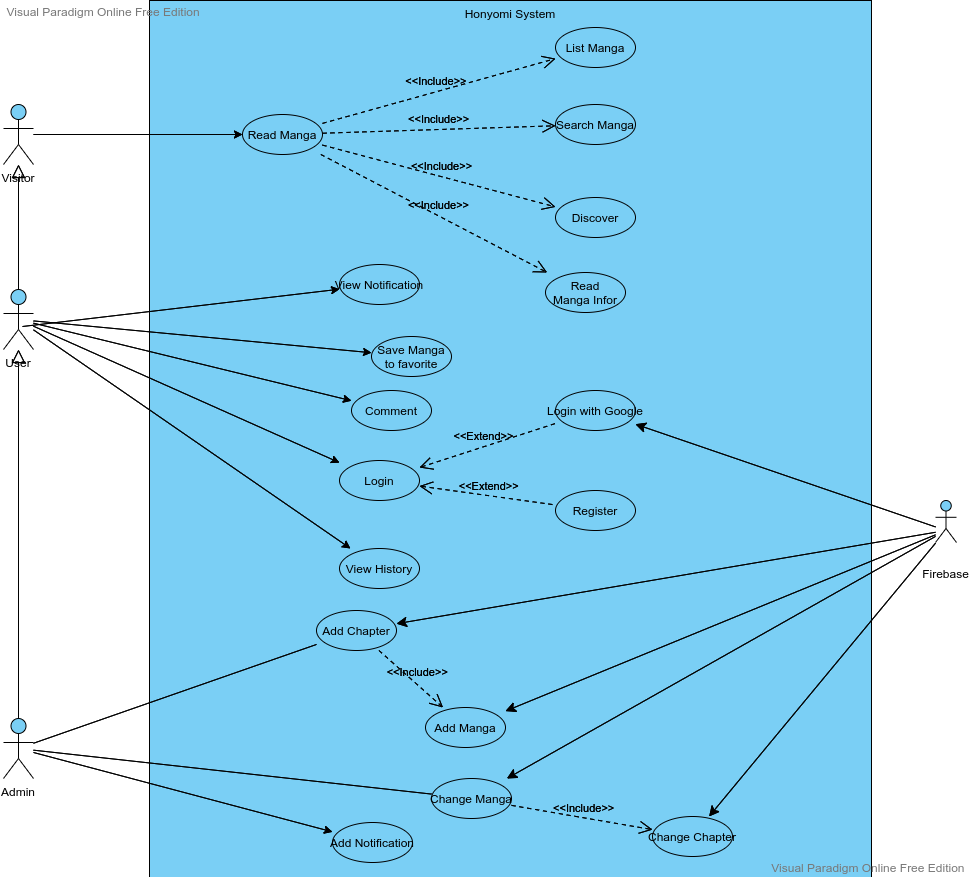
\includegraphics[width=\linewidth]{./images/image6.png}
	\caption{Biểu đồ ca sử dụng}
\end{figure}

\end{document}